\begin{frame}{Ευθυγράμμιση πανοραμικών σαρώσεων από ευθυγράμμιση εικόνων}


  \begin{figure}
    
\definecolor{r}{RGB}{255 0 0}
\definecolor{g}{RGB}{0 155 0}
\definecolor{b}{RGB}{0 0 255}

\tikzset{every picture/.style={line width=0.75pt}} %set default line width to 0.75pt

\begin{tikzpicture}[x=0.75pt,y=0.75pt,yscale=-1,xscale=1]
%uncomment if require: \path (0,442); %set diagram left start at 0, and has height of 442

%Image [id:dp7345435744663564]
\draw (40.99,137.25) node  {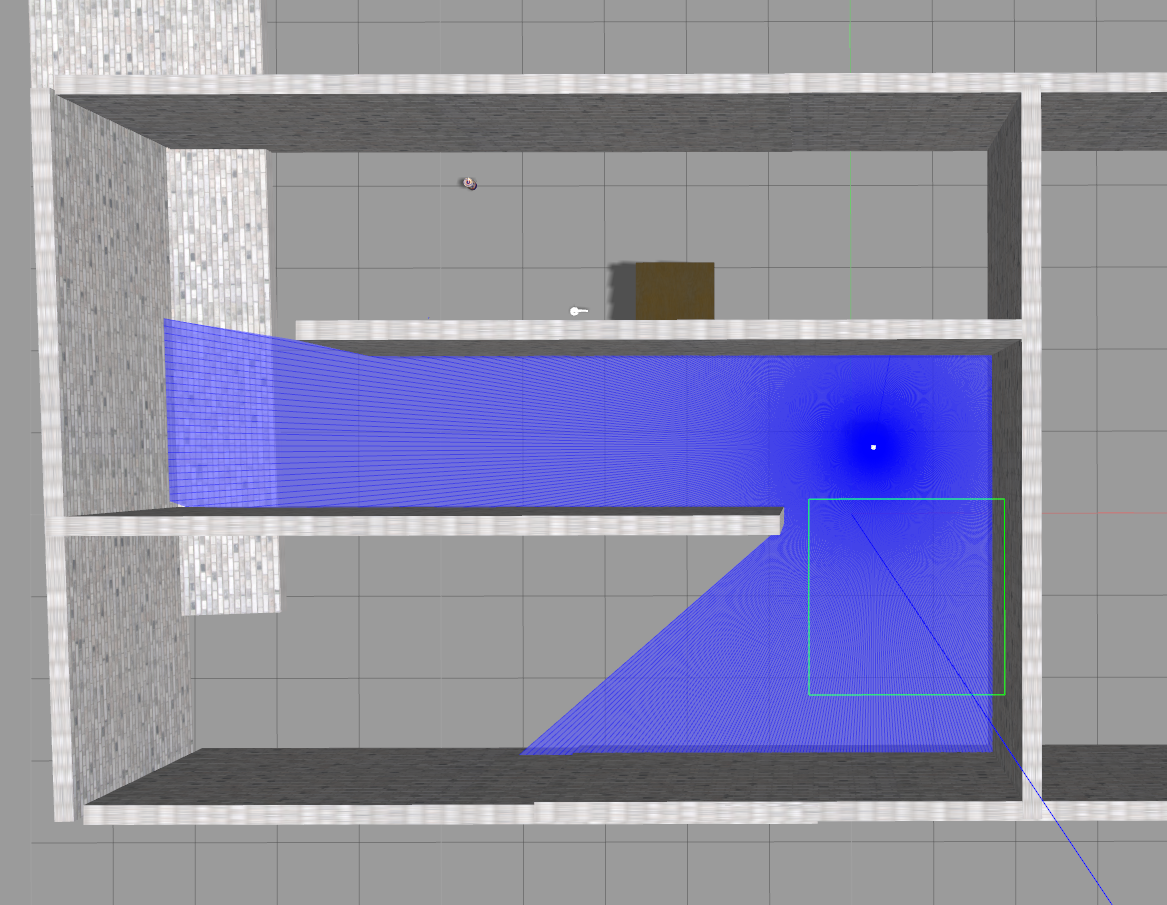
\includegraphics[width=52.5pt,height=40.71pt]{./figures/slides/ch5/scan_to_image/env.png}};
%Image [id:dp030872284892191182]
\draw (40.99,217.99) node  {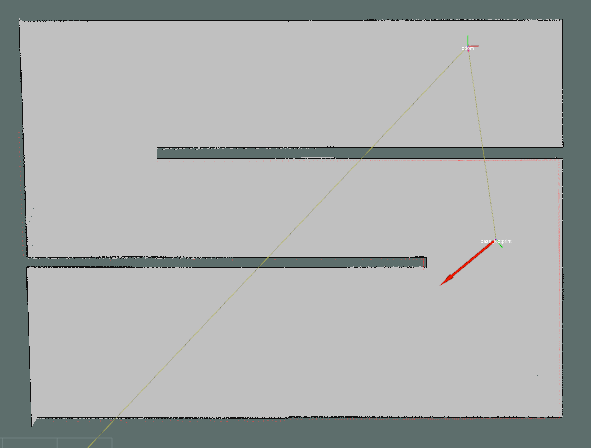
\includegraphics[width=52.5pt,height=39.8pt]{./figures/slides/ch5/scan_to_image/map.png}};
%Image [id:dp9855156395144604]
\draw (140.99,217.99) node  {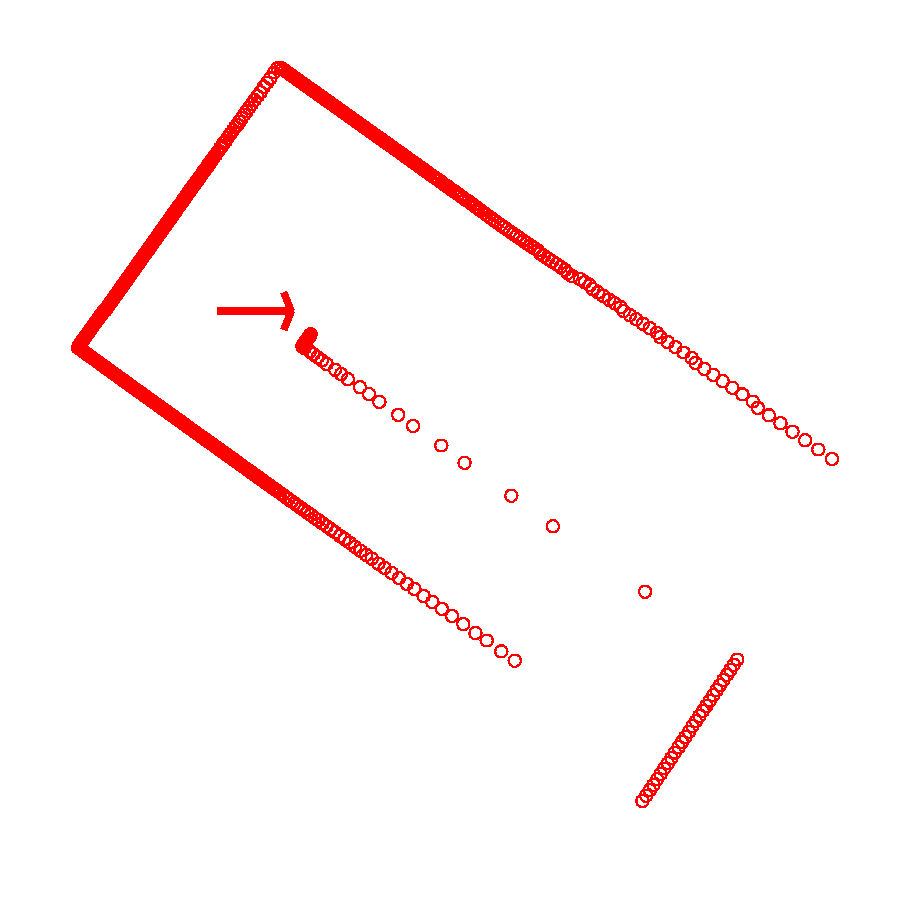
\includegraphics[width=52.5pt,height=52.5pt]{./figures/slides/ch5/scan_to_image/sv.png}};
%Image [id:dp0883330060973122]
\draw (140.49,137.25) node  {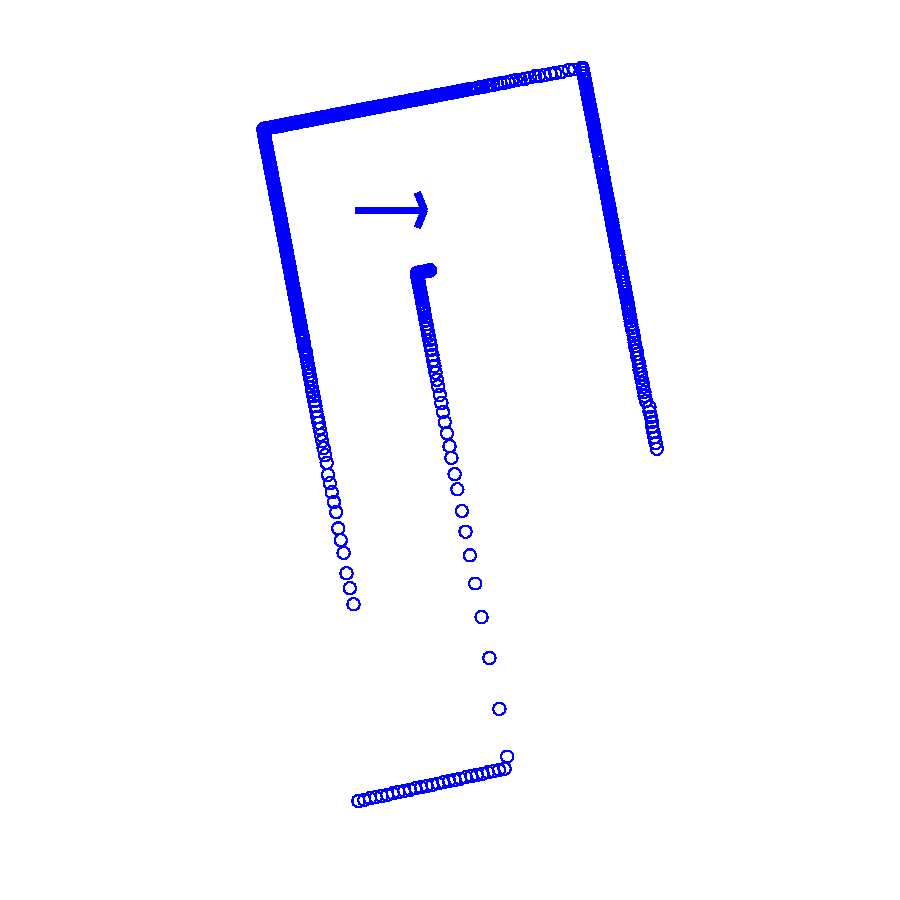
\includegraphics[width=52.5pt,height=52.5pt]{./figures/slides/ch5/scan_to_image/sr.png}};
%Image [id:dp8079986507529633]
\draw (240.49,137.25) node  {
\includegraphics[width=52.5pt,height=52.5pt]{./figures/slides/ch5/scan_to_image/real.png}};
%Image [id:dp04118937468211392]
\draw (238.99,217.99) node  {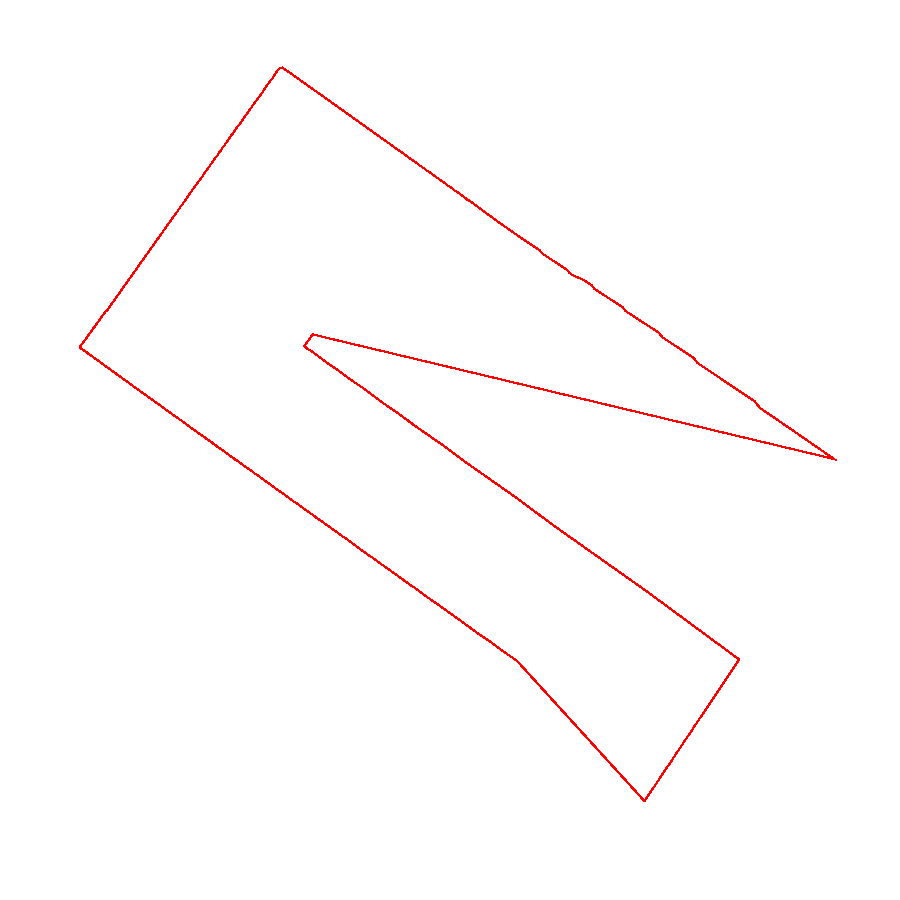
\includegraphics[width=52.5pt,height=52.5pt]{./figures/slides/ch5/scan_to_image/virtual.png}};
%Straight Lines [id:da3336180290494899]
\draw    (274,137.25) -- (322.75,137.25) ;
%Straight Lines [id:da6380620434779032]
\draw    (274,217.99) -- (322.75,217.99) ;
%Straight Lines [id:da15384576533302807]
\draw    (322.75,137.25) -- (322.75,161.25) ;
\draw [shift={(322.75,163.25)}, rotate = 270] [color={rgb, 255:red, 0; green, 0; blue, 0 }  ][line width=0.75]    (10.93,-3.29) .. controls (6.95,-1.4) and (3.31,-0.3) .. (0,0) .. controls (3.31,0.3) and (6.95,1.4) .. (10.93,3.29)   ;
%Straight Lines [id:da8338083407403734]
\draw    (322.75,218.99) -- (322.75,193.93) ;
\draw [shift={(322.75,191.93)}, rotate = 90] [color={rgb, 255:red, 0; green, 0; blue, 0 }  ][line width=0.75]    (10.93,-3.29) .. controls (6.95,-1.4) and (3.31,-0.3) .. (0,0) .. controls (3.31,0.3) and (6.95,1.4) .. (10.93,3.29)   ;
%Straight Lines [id:da31631966071327233]
\draw    (375.35,177.29) -- (436.85,177.29) -- (436.85,163) ;
%Straight Lines [id:da7038147916669211]
\draw    (355.39,189.38) -- (355.39,261.38) ;
\draw [shift={(355.39,263.38)}, rotate = 270] [color={rgb, 255:red, 0; green, 0; blue, 0 }  ][line width=0.75]    (10.93,-3.29) .. controls (6.95,-1.4) and (3.31,-0.3) .. (0,0) .. controls (3.31,0.3) and (6.95,1.4) .. (10.93,3.29)   ;
%Image [id:dp4359687414115401]
\draw (438.1,113.14) node  {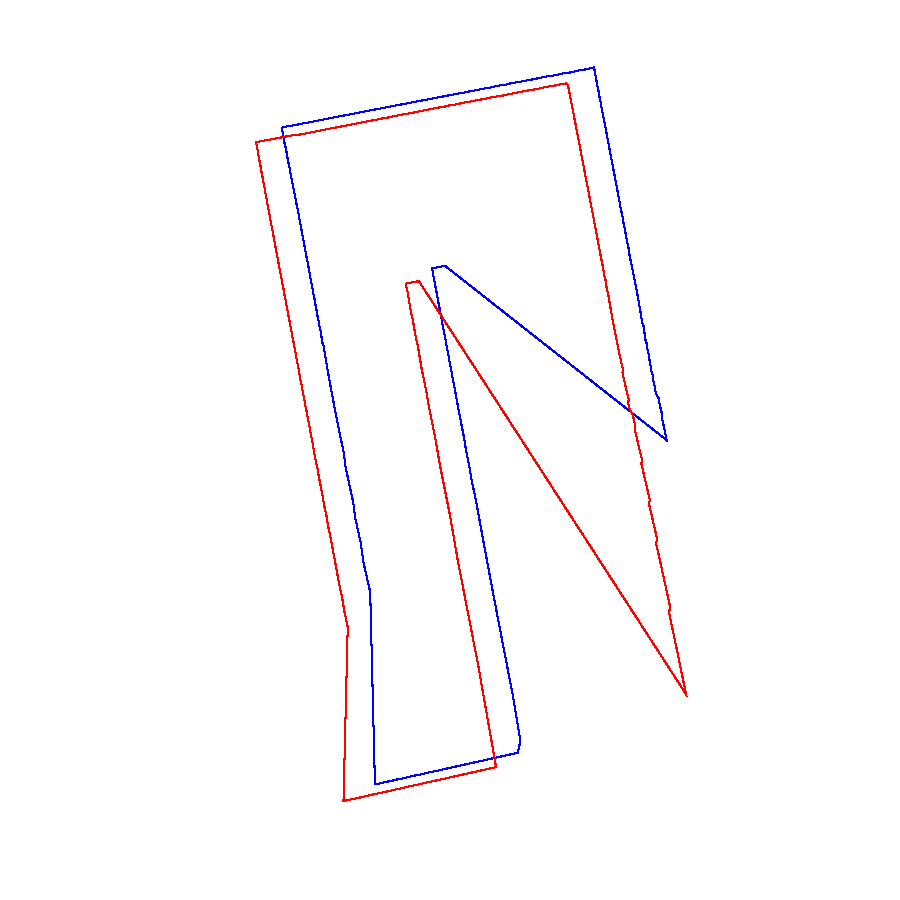
\includegraphics[width=74.86pt,height=74.86pt]{./figures/slides/ch5/scan_to_image/aligned.png}};
%Straight Lines [id:da4365786762663775]
\draw    (77.39,137.25) -- (101.89,137.25) ;
\draw [shift={(103.89,137.25)}, rotate = 180] [color={rgb, 255:red, 0; green, 0; blue, 0 }  ][line width=0.75]    (10.93,-3.29) .. controls (6.95,-1.4) and (3.31,-0.3) .. (0,0) .. controls (3.31,0.3) and (6.95,1.4) .. (10.93,3.29)   ;
%Straight Lines [id:da9500470672515446]
\draw    (77.39,217.99) -- (101.89,217.99) ;
\draw [shift={(103.89,217.99)}, rotate = 180] [color={rgb, 255:red, 0; green, 0; blue, 0 }  ][line width=0.75]    (10.93,-3.29) .. controls (6.95,-1.4) and (3.31,-0.3) .. (0,0) .. controls (3.31,0.3) and (6.95,1.4) .. (10.93,3.29)   ;
%Straight Lines [id:da18131060303921864]
\draw    (175.89,137.25) -- (200.39,137.25) ;
\draw [shift={(202.39,137.25)}, rotate = 180] [color={rgb, 255:red, 0; green, 0; blue, 0 }  ][line width=0.75]    (10.93,-3.29) .. controls (6.95,-1.4) and (3.31,-0.3) .. (0,0) .. controls (3.31,0.3) and (6.95,1.4) .. (10.93,3.29)   ;
%Straight Lines [id:da16835710408982396]
\draw    (175.89,217.99) -- (200.39,217.99) ;
\draw [shift={(202.39,217.99)}, rotate = 180] [color={rgb, 255:red, 0; green, 0; blue, 0 }  ][line width=0.75]    (10.93,-3.29) .. controls (6.95,-1.4) and (3.31,-0.3) .. (0,0) .. controls (3.31,0.3) and (6.95,1.4) .. (10.93,3.29)   ;
%Image [id:dp9297806524160088]
\draw (438.1,240.49) node  {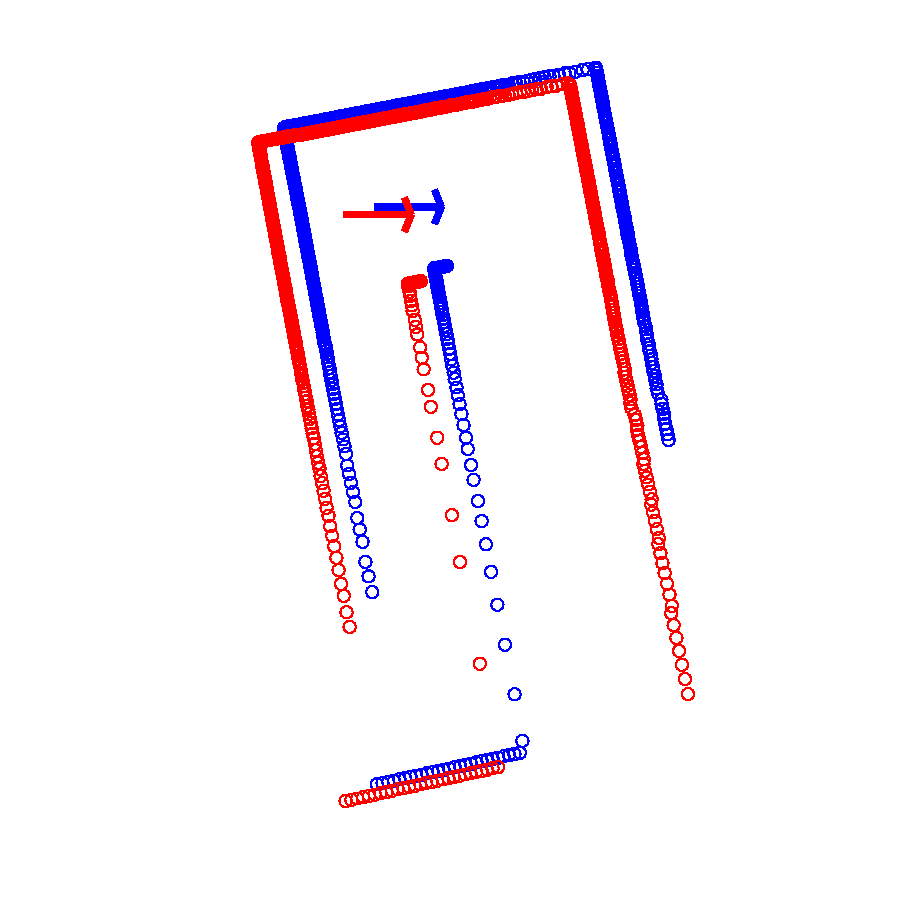
\includegraphics[width=75.38pt,height=75.38pt]{./figures/slides/ch5/scan_to_image/s_aligned.png}};
%Shape: Rectangle [id:dp41358298385049075]
\draw   (5.99,110.1) -- (75.99,110.1) -- (75.99,164.39) -- (5.99,164.39) -- cycle ;
%Shape: Rectangle [id:dp8289234142790565]
\draw   (5.99,191.46) -- (75.99,191.46) -- (75.99,244.52) -- (5.99,244.52) -- cycle ;
%Shape: Rectangle [id:dp5428699224303526]
\draw   (105.49,102.25) -- (175.89,102.25) -- (175.89,172.25) -- (105.49,172.25) -- cycle ;
%Shape: Rectangle [id:dp42147633315554844]
\draw   (105.99,182.99) -- (175.89,182.99) -- (175.89,252.99) -- (105.99,252.99) -- cycle ;
%Shape: Rectangle [id:dp6049360628407487]
\draw   (205.49,102.25) -- (274,102.25) -- (274,172.25) -- (205.49,172.25) -- cycle ;
%Shape: Rectangle [id:dp2521020767932107]
\draw   (203.99,182.99) -- (274,182.99) -- (274,252.99) -- (203.99,252.99) -- cycle ;
%Shape: Rectangle [id:dp6142215604413235]
\draw   (388.19,63.23) -- (488.01,63.23) -- (488.01,163.05) -- (388.19,163.05) -- cycle ;
%Shape: Rectangle [id:dp9231570758043264]
\draw   (388.35,190.66) -- (487.85,190.66) -- (487.85,296.23) -- (388.35,296.23) -- cycle ;
%Straight Lines [id:da1181254794306934]
\draw [color={rgb, 255:red, 126; green, 211; blue, 33 }  ,draw opacity=1, dotted ]   (436.85,177.29) -- (436.85,190.5) ;

% Text Node
\draw    (283.16,165) -- (375.35,165) -- (375.35,190) -- (283.16,190) -- cycle  ;
\draw (329.16,177.5) node   [align=left] {\texttt{FMI\_SPOMF}};
% Text Node
\draw (274,276) node [anchor=north west][inner sep=0.75pt]   [align=left] {\small \sout{$(\Delta x, \Delta_y)$}, $\Delta \theta$, \textcolor{g}{$\sigma$}, $w$};
% Text Node
\draw (7, 49.5) node [anchor=north west][inner sep=0.75pt]   [align=left] {Περιβάλλον};
\draw (34,69.5) node [anchor=north west][inner sep=0.75pt]   [align=left] {+};
\draw (14,86.5) node [anchor=north west][inner sep=0.75pt]   [align=left] {Σάρωση};
% Text Node
\draw (16,267) node [anchor=north west][inner sep=0.75pt]   [align=left] {Χάρτης};
\draw (33,287) node [anchor=north west][inner sep=0.75pt]   [align=left] {+};
\draw (10,304) node [anchor=north west][inner sep=0.75pt]   [align=left] {Εκτίμηση};
% Text Node
\draw (121,77.39) node [anchor=north west][inner sep=0.75pt]   [align=left] {$\mathcal{S}_R(\bm{p})$};
% Text Node
\draw (121,266.5) node [anchor=north west][inner sep=0.75pt]   [align=left] {$\mathcal{S}_V(\hat{\bm{p}})$};
% Text Node
\draw (231,78.5) node [anchor=north west][inner sep=0.75pt]   [align=left] {$\texttt{I}_R$};
% Text Node
\draw (231,266.5) node [anchor=north west][inner sep=0.75pt]   [align=left] {$\texttt{I}_V$};
% Text Node
\draw (412.1,44) node [anchor=north west][inner sep=0.75pt]   [align=left] {\textcolor{b}{$\texttt{I}_R$}, \textcolor{r}{$\texttt{I}_V^{\text{rot}}$}};
% Text Node
\draw (385.1,300) node [anchor=north west][inner sep=0.75pt]   [align=left] {\textcolor{b}{$\mathcal{S}_R$}(\textcolor{b}{$\bm{p}$}), \textcolor{r}{$\mathcal{S}_V^{\text{rot}}$}(\textcolor{r}{$\hat{\bm{p}}^{\text{rot}}$})};

\draw [draw=white, fill=white, opacity=0.9] (177,44) -- (512,44) -- (512,320) -- (177,320) -- cycle;

\end{tikzpicture}


  \end{figure}


\note{\footnotesize
Ας υποθέσουμε λοιπόν πως έχουμε στη διάθεσή μας μία πανοραμική σάρωση $S_R$,
το χάρτη του περιβάλλοντος, και μία εκτίμηση για τη στάση του αισθητήρα lidar.
Μέσω της εκτίμησης και του χάρτη είναι δυνατός ο υπολογισμός της εικονικής
σάρωσης $S_V$ μέσω raycasting.}


\end{frame}
